\documentclass{article}

\makeatletter
\renewcommand{\fnum@figure}{Εικόνα \thefigure}
\makeatother

\usepackage[greek, english]{babel}
\usepackage{alphabeta}
\usepackage{atbegshi, picture}

% Set page size and margins
% Replace `letterpaper' with`a4paper' for UK/EU standard size
\usepackage[letterpaper,top=2cm,bottom=2cm,left=3cm,right=3cm,marginparwidth=1.75cm]{geometry}

% Useful packages
\usepackage{amsmath}
\usepackage{graphicx}
\usepackage[colorlinks=true, allcolors=blue]{hyperref}
\usepackage[utf8]{inputenc}
\usepackage{indentfirst}

\newcommand\T{\rule{0pt}{2.6ex}}       % Top strut
\newcommand\B{\rule[-1.2ex]{0pt}{0pt}} 


\addto\captionsenglish{
  \renewcommand{\contentsname}
    {Περιεχόμενα}
}

% \title{Feasibility Study}
% \date{}

\begin{document}
% \maketitle

\begin{titlepage}
   \begin{center}
       \vspace*{1cm}

       \textbf{\huge Use Cases}

       \vspace{0.5cm}
        Τεχνολογία Λογισμικού
            
       \vspace{1cm}

       \textbf{Αγγελική Κούρου\\Κατερίνα Μητροπούλου\\Μάριος Στεφανίδης}
       
       \begin{figure}[!htb]
        \centering
        
\includegraphics[width=0.5\textwidth]{logo.png}
        \end{figure}
        
        \vspace{0.5cm}
        
        \begin{figure}[!htb]
        \centering
        \includegraphics[width=0.5\textwidth]{UoP.jpg}
        \end{figure}


       \vfill
            
       Τεχνικό Κείμενο για την Τεχνολογία Λογισμικού\\
            
       \vspace{0.5cm}
            
       CEID, ECE\\
       University of Patras\\
            
   \end{center}
\end{titlepage}



\noindent Η ομάδα μας

\begin{enumerate}
  \item Βεργίνης Δημήτριος, ΑΜ: 10166634 , ECE
  \item Βλαχογιάννης Δημήτριος, ΑΜ: 1067371, CEID
  \item Κούρου Αγγελική, ΑΜ: 1067499 , CEID
  \item Μητροπούλου Αικατερίνα - Quality Manager, ΑΜ: 1067409, CEID
  \item Στεφανίδης Μάριος - Project Manager, ΑΜ:1067458, CEID
\end{enumerate}

{
  \hypersetup{linkcolor=black}
  \tableofcontents
}

\section{Εισαγωγή}

Τα Use Cases αποτελούν ένα σύνολο δραστηριοτήτων ή των βημάτων που λαμβάνουν χώρα κατά την πλοήγηση ενός χρήστη (ή ρόλου - γνωστού στην UML ως ηθοποιού) σε ένα σύστημα, για να επιτευχθεί ένας στόχος. Ο ηθοποιός μπορεί να είναι άνθρωπος ή κάποιο άλλο εξωτερικό σύστημα. 
Για την ανάπτυξη ενός use case χρησιμοποιούνται τα διαγράμματα περιπτώσεων χρήσης, καθώς και λεκτική περιγραφή των περιπτώσεων αυτών.

\section{Διάγραμμα Περιπτώσεων Χρήσης}

Παρακάτω παρουσιάζεται το διάγραμμα περιπτώσεων χρήσης. Για την καλύτερη κατανόηση του διαγράμματος σημειώνεται ότι:

\begin{enumerate}
  \item Τα σκίτσα με τους ανθρώπους αντιστοιχούν στους ηθοποιούςτ του εκάστοτε use case, δηλαδή τους εμπλεκόμενους
  \item Οι μπλε ελλείψεις αντιστοιχούν στα use cases
  \item Οι μαύρες γραμμές απεικονίζουν άμεση συσχέτιση μεταξύ ενός ηθοποιού και μίας περίπτωησης χρήσης
  \item Οι μαύρες διακεκομμένες γραμμές απεικονίζουν τη σχέση εξάρτησης μεταξύ δύο περιπτώσεων χρήσης, δηλαδή το use case στο οποίο δείχνει το βέλος δεν μπορεί να υπάρξει αν δεν έχει προηγηθεί το use case από το οποίο ξεκινάει το βέλος  
\end{enumerate}


\newpage
\begin{figure}[!htb]
        \centering
        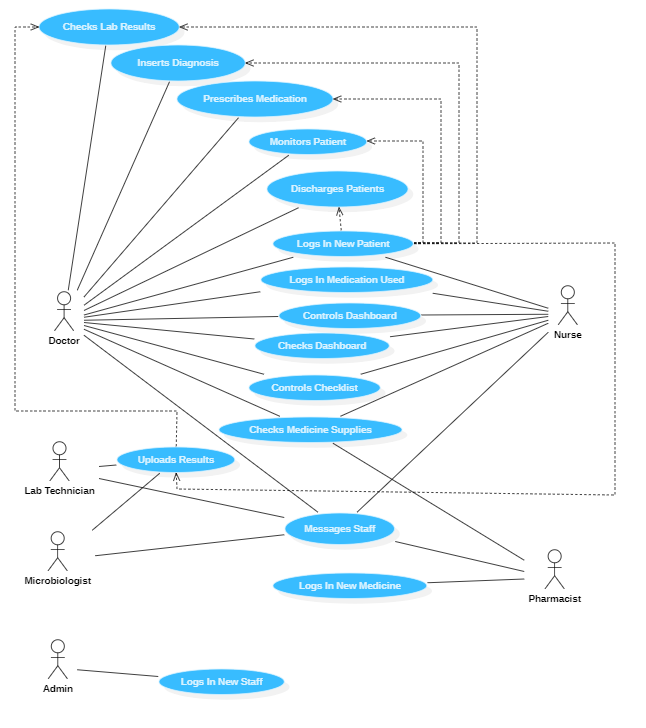
\includegraphics[width=0.5\textwidth]{UML.png}
        \end{figure}
        
        \vspace{0.5cm}

\section{Use Case 1: Monitoring Ασθενούς}

Παρακάτω θα αναλυθεί το σενάριο χρήσης του \textbf{Medic World} κατά το οποίο ένας γιατρός επιθυμεί να προσθέσει διάγνωση στην καρτέλα ενός ασθενούς.

\subsection{Περιγραφή}

\begin{center}
     \begin{tabular}{|l|l|}
     \hline
      \textbf{Περίπτωση Χρήσης 1 }   & Ο γιατρός ελέγχει την κατάσταση ενός ασθενούς \T\B \\ 
      \hline
      \textbf{Ηθοποιός} & Γιατρός \T\B \\
      \hline
      \textbf{Σενάριο Περίπτωσης Χρήσης} & Μία από τους ασθενής χρείαζεται διάγνωση, οπότε\\& ο γιατρός εισέρχεται στην καρτέλα της, μελετάει τα\\& αποτελέσματα των εξετάσεών της και καταλήγει σε διάγνωση\T\B \\
      \hline
      \textbf{Αφορμή} & Ασθενής χρειάζεται διάγνωση \T\B \\
      \hline
      \textbf{Προαπαιτούμενο 1} & Να έχει καταχωρηθεί ο ασθενής \T\B \\
      \hline
      \textbf{Ποραπαιτούμενο 2} & Να έχουν βγει τα αποτελέσματα των εργαστηριακών εξετάσεων \T\B \\
      \hline
     \end{tabular}
 \end{center}
 
 \subsection{Αναλυτικό Σενάριο Χρήσης}
 
 \begin{center}
     \begin{tabular}{|l|l|}
     \hline
      \textbf{Περιγραφή }   & Αυτό το σενάριο περιγράφει μια κατάσταση όπου χρείαζεται\\& η πλοήγηση σε τέσσερις καρτέλες. Αυτές οι τέσσερις\\& οδηγούν στη επιτυχία του στόχου. \T\B \\ 
      \hline
      \textbf{1} & Ο γιατρός από το κεντρικό μενού επιλέγει το εικονίδιο\\& "Patients" \T\B \\
      \hline
      \textbf{2} & Ο γιατρός επιλέγει τον ασθενή που χρειάζεται διάγνωση\T\B \\
      \hline
      \textbf{3} & Ο γιατρός εξετάζει την κατάσταση του ασθενούς \T\B \\
      \hline
      \textbf{4} & Ο γιατρός εξετάζει το ιστορικό του ασσθενούς \T\B \\
      \hline
      \textbf{5} & Ο γιατρός επιλέγει τα "lab results" \T\B \\
      \hline
      \textbf{6} & Ο γιατρός μελετάει τα "lab results" \T\B \\
      \hline
      \textbf{7} & Ο γιατρός επιλέγει το πλήκτρο για νέα διάγνωση \T\B \\
      \hline
      \textbf{8} & Ο γιατρός εισάγει τη νέα διάγνωση \T\B \\
      \hline
      \textbf{9} & Ο γιατρός επιλέγει το πλήκτρο ολοκλήρωσης \T\B \\
      \hline
      \textbf{10} & Στην καρτέλα του ασθενούς εμφανίζεται η διάγνωση \T\B \\
      \hline
     \end{tabular}
 \end{center}
 
 
 \section{Use Case 1: Απασχόληση Χειρουργείου}
 
 Παρακάτω θα αναλυθεί το σενάριο χρήσης του \textbf{Medic World} κατά το οποίο ένας χρήστης επιθυμεί να δηλώσει στο σύστημα τη χρήση ενός χειρουργείου.

\subsection{Περιγραφή}

\begin{center}
     \begin{tabular}{|l|l|}
     \hline
      \textbf{Περίπτωση Χρήσης 2 }   & Ο χρήστης δηλώνει τη χρήση χειρουργείου\T\B \\ 
      \hline
      \textbf{Ηθοποιός} & Γιατρός \T\B \\
      \hline
      \textbf{Σενάριο Περίπτωσης Χρήσης} & Ένας γιατρός πρόκειται να εισάγει έναν ασθενή\\& σε κάποιο χειρουργείο και χρειάζεται να καταχωρηθεί\\& στην καρτέλα των χειρουργείων, ότι το συγκεκριμένο\\& δωμάτιο δε θα είναι πλέον διαθέσιμο\T\B \\
      \hline
      \textbf{Ηθοποιοί} & Γιατρός, Νοσηλευτής \T\B \\
      \hline
      \textbf{Αφορμή} & Ασθενής χρειάζεται χειρουργείο\T\B \\
      \hline
      \textbf{Προαπαιτούμενο 1} & Να έχει καταχωρηθεί ο ασθενής \T\B \\
      \hline
      \textbf{Πρoαπαιτούμενο 2} & Να έχει πραγματοποιηθεί διάγνωση του ασθενούς \T\B \\
      \hline
      \textbf{Προαπαιτούμενο 3} & Η διάγνωση να απαιτεί την εισαγωγή σε χειρουργείο \T\B \\
      \hline
     \end{tabular}
 \end{center}
 
 \subsection{Αναλυτικό Σενάριο Χρήσης}
 
 \begin{center}
     \begin{tabular}{|l|l|}
     \hline
      \textbf{Περιγραφή }   & Αυτό το σενάριο περιγράφει μια κατάσταση όπου χρείαζεται\\& η πλοήγηση σε τέσσερις καρτέλες. Αυτές οι τέσσερις\\& οδηγούν στη επιτυχία του στόχου. \T\B \\ 
      \hline
      \textbf{1} & Ο χρήστης επιλέγει από το κεντρικό μενού το εικονίδιο\\& "Checklist" \T\B \\
      \hline
      \textbf{2} & Ο χρήστης επιλέγει από το μενού του Checklist\\& τα "Operating Rooms" \T\B \\
      \hline
      \textbf{3} & Ο χρήστης ελέγχει τη διαθεσιμότητα των χειρουργείων \T\B \\
      \hline
      \textbf{4} & Ο χρήστης επιλέγει ένα από τα διαθέσιμα χειρουργεία \T\B \\
      \hline
      \textbf{5} & Ο χρήστης οδηγείται σε μία φόρμα συμπλήρωσης στοιχείων \T\B \\
      \hline
      \textbf{6} & Ο χρήστης εισάγει τα στοιχεία που απαιτεί η φόρμα\T\B \\
      \hline
      \textbf{7} & Ο ο χρήστης μέσω του πλήκτρου "Done" επιλέγει την\\& ολοκλήρωση της διαδικασίας \T\B \\
      \hline
      \textbf{8} & Στην καρτέλα διαθεσιμότητας των χειρουργείων\\& εμφανίζεται πλέον ως μη διαθέσιμο το χειρουργείο\\& που επέλεξε νωρίτερα ο χρήστης \T\B \\
      \hline
     \end{tabular}
 \end{center}

\end{document}
